\documentclass{jfm}

% Compilation
\usepackage{silence} % Silence latex compiler warnings
\WarningFilter{latex}{Command \@xhline has changed} % Filter out warning
  % caused by redefinition between jfm.cls class and array (loaded by
  % siunitx)

% Import custom style file containing common packages and options
\setlength{\paperheight}{\pdfpageheight} % JFM class removes paperheight definition and hyperref raises a warning

% Import custom style file containing common packages and options
\usepackage{preamble}
\graphicspath{{./Figures/}}

% Discrete Fourier Transform
\newcommand{\GenP}{\hat{P}_m}
\newcommand{\POne}{\hat{P}_1}
\newcommand{\PTwo}{\hat{P}_2}
\newcommand{\PThree}{\hat{P}_3}
\newcommand{\PFour}{\hat{P}_4}

% Continuous Fourier Transform
\newcommand{\GenPk}{\hat{P} (\kappa)}
\newcommand{\PZerok}{\hat{P} (0)}

% Define custom math symbols
\DeclareMathOperator{\cn}{Cn}
\DeclareMathOperator{\sgn}{sgn}
\DeclareMathOperator{\Ur}{Ur}
\DeclareMathOperator{\Sk}{Sk}
\DeclareMathOperator{\As}{As}
%\DeclareMathOperator{\Bi}{Bi}

\newcommand{\hilbert}{\mathcal{H}}

% Define custom math functions
\DeclarePairedDelimiter{\round}{\lfloor}{\rceil}

% Define \im as Roman i
\newcommand{\im}{\mathrm{i}}
% Replace epsilon with varepsilon
\renewcommand*{\epsilon}{\varepsilon}

%% Use \thalf and \squart commands from JFM class
%\newcommand\squart{\ensuremath{{\textstyle\frac{1}{4}}}}
%\newcommand\thalf{\ensuremath{{\textstyle\frac{1}{2}}}}

\linenumbers{}

\title{Wind-Induced Changes to Surface Gravity Wave Shape in Shallow Water}

\author{Thomas J. Zdyrski \and Falk Feddersen}

\begin{document}

\maketitle

\begin{abstract}
Wave shape (\eg{} wave skewness and asymmetry) impacts sediment
transport, remote sensing and ship safety.
Previous work showed that wind affects wave shape in intermediate and
deep water.
Here, we investigate the effect of wind on wave shape in shallow water
through a wind-induced surface pressure for different wind speeds and
directions.
A multiple-scale analysis of long waves propagating over a shallow,
flat bottom and forced by a Jeffreys-type surface pressure produces a
Korteweg-de Vries (KdV)-Burgers equation for the wave profile.
The wave evolution of an symmetric, solitary wave initial condition is
calculated numerically.
The resulting wave grows (decays) for onshore (offshore) wind and
becomes asymmetric, with the rear face showing the largest shape
changes.
Additionally, the result's deviation from a reference solitary wave
shows an bound, dispersive tail.
The onshore wind increases the wave's energy and skewness with time
while decreasing the wave's asymmetry, with the opposite holding for
offshore wind.
The corresponding wind speeds are shown to be physically realistic, and
the shape changes are explained as slow growth followed by rapid
evolution according to the unforced KdV equation.
\end{abstract}

\vspace{-0.7cm}
\section{Introduction}

The study of wind and ocean wave interactions began with
\citet{jeffreys1925formation} and continues to be an active field of
research~\citep[\eg][]{janssen1991quasi,donelan2006wave,sulivan2010dynamics}.
Many theoretical
studies~\citep[\eg][]{jeffreys1925formation,miles1957generation,phillips1957generation}
focus on calculating wind-induced growth rates and often employ
phase-averaging techniques.
However, wind can also influence wave shape, quantified by third-order
shape statistics such as skewness and asymmetry, corresponding to
vertical and horizontal asymmetry,
respectively~\citep[\eg][]{leykin1995asymmetry,feddersen2005wind,zdyrski2020wind}.
Wave shape influences sediment transport and modulates beach
morphodynamics~\citep[\eg][]{drake2001discrete,hoefel2003wave}, while
wave skewness affects radar altimetry
signals~\citep[\eg][]{hayne1980radar} and asymmetry modulates ship
responses to wave impacts~\citep[\eg][]{soares2008abnormal}.

Waves in shallow water, where $kh \ll 1$ (with $h$ the water depth and
$k=2\pi/\lambda$ the wavenumber), differ qualitatively from those in
intermediate to deep water where $kh \sim 1$ or $\gg 1$, respectively.
For waves with small amplitudes $a_0 \ll h$,
leveraging the small parameters $a_0/h \sim (kh)^2 \ll 1$
yields the Boussinesq equations with weak dispersion and nonlinearity.
A special class of waves formed when dispersion balances nonlinear
focusing are known as solitary waves and appear in environments ranging
from nonlinear optical pulses \citep[\eg][]{kivshar1993dark} to
astrophysical dusty plasmas \citep[\eg][]{sahu2012nonextensive}.
One of the simplest equations displaying solitary waves is the
Korteweg-de Vries (KdV) equation, which incorporates dispersion and
nonlinearity.
When augmented with a dissipative term, this becomes the KdV-Burgers
equation, with applications to damped internal tides
\citep[\eg][]{sandstrom1995dissipation}, electron waves in graphene
\citep[\eg][]{zdyrski2019effects} and viscous flow in blood vessels
\citep[\eg][]{antar1999weakly}.
To investigate wind and surface wave interactions in shallow water, we
introduce a wind-induced pressure term to the Boussinesq equations in
\cref{sec:derivation}.
The resulting KdV-Burgers equation governs a solitary wave's evolution,
which we solve numerically to yield the wave energy, skewness and
asymmetry in \cref{sec:results}.
We calculate the wind speed, discuss the asymmetry and
compare our results to intermediate- and deep-water waves in
\cref{sec:discussion}.

\vspace{-0.5cm}
\section{\label{sec:derivation} Derivation of the KdV-Burgers equation}

\subsection{Governing equations}
We treat the flow as irrotational and inviscid and neglect surface
tension by considering length scales much greater than
\SI{2}{\centi\meter}.
Furthermore, we restrict to planar wave propagation in the $+x$
direction.
Finally, we choose a coordinate system with $z=0$ at the mean water
level and a horizontal, flat bottom located at $z=-h$.
Then, the incompressibility condition and standard boundary conditions
are
\begin{alignat}{2}
  0 &= \phi_{xx} + \phi_{zz} &&\qq{on}
  -h < z < \eta \,, \label{eq:laplace}\\
  0 &= \phi_{z} &&\qq{on} z=-h \,, \label{eq:bottom_bc}\\
  \phi_{z} &= \eta_{t} + \phi_{x} \eta_{x} &&\qq{on} z = \eta \,,
  \label{eq:kinematic_bc}\\
  0 &= \frac{p}{\rho_w} + g\eta + \phi_{t} +
  \frac{1}{2} \bqty{\phi_{x}^2 + \phi_{z}^2} &&\qq{on} z=
  \eta \,. \label{eq:dynamic_bc}
\end{alignat}
Here, $\eta(x,t)$ is the wave profile, $\phi(x,z,t)$ is the flow's
velocity potential related to the velocity $\vec{u} = \grad{\phi}$,
$p(x,t)$ is the surface pressure, $g$ is the gravitational acceleration
and $\rho_w$ is the water density.
We used $\phi$'s gauge freedom to absorb the Bernoulli `constant'
$C(t)$ in the dynamic boundary condition.
We are seeking a solitary, progressive wave which decays at infinity,
$\eta(\vec{x},t) \to 0$ as $\abs{\vec{x}} \to \infty$, with similar
conditions on $\vec{u}$.
We choose a coordinate system where the average bottom horizontal
velocity vanishes,
\begin{equation}
  \overline{ \pdv{\phi}{x} } = 0 \qq{on} z=-h \,,
  \label{eq:bot_bc_horz}
\end{equation}
with the overline a spatial average $\overline{f} \coloneqq
\lim_{L\to\infty} \int_{-L}^{L} f \dd{x} / (2L)$.
Additionally, we assume the surface pressure $p(x,t)$ is a Jeffreys-type
forcing \citep{jeffreys1925formation},
\begin{equation}
  p(x,t) = P \pdv{\eta(x,t)}{x} \,.
\end{equation}
Here, $P$ is proportional to $(U-c)^2$, with $c$ the phase speed and $U$
the wind speed (\cf{} \cref{sec:press_mag}), and $P>0$ corresponds to
(`onshore') wind in the same direction as the wave while $P<0$ denotes
(`offshore') wind opposite the wave.
We use a Jeffreys forcing for its analytic simplicity and clear
demonstration of wind-wave coupling.
Jeffrey's separated sheltering mechanism is likely only relevant
in special situations (\eg{} near breaking,
\citealp{banner1976separation}, or for steep waves under strong winds,
\citealp{tian2013evolution,touboul2006interaction}).
Numerical simulations of sinusoidal waves suggest the peak surface
pressure is shifted approximately \SI{135}{\degree} from the wave peak,
while Jeffreys would give a \SI{90}{\degree}
shift~\citep{husain2019boundary}.
A fully dynamic coupling between wind and waves---necessary for an
accurate surface pressure over a non-sinusoidal, dynamic water
surface---is outside the scope of this paper.

\subsection{\label{sec:nondim} Non-dimensionalization}
We non-dimensionalize our system with the known characteristic
scales: the horizontal length scale $L$ over which $\eta$ changes
rapidly, expressed as an effective wavenumber $k_E \coloneqq 2 \pi/L$;
the (initial) wave amplitude $a_0 = H_0/2$ (\ie{} half the wave height
$H_0$); the depth $h$; the gravitational acceleration $g$; and the wind
speed $U$, expressed as a pressure magnitude $P \propto \rho_a (U-c)^2$.
Denoting non-dimensional variables with primes, we have
\begin{equation}
  \begin{aligned}
  x &= \frac{x'}{k_E} = h \frac{x'}{\sqrt{\mu_E}}\,, \\
  z &= h z' \,,
  \end{aligned}
  \qquad
  \begin{aligned}
  t &= \frac{t'}{k_E\sqrt{g h}}
    = \frac{t'}{\sqrt{\mu_E}} \sqrt{\frac{h}{g}} \,, \\
  P &= \epsilon P' \frac{\rho_w g}{k_E}
    = \frac{\epsilon}{\sqrt{\mu_E}} P' \rho_w g h \,,
  \end{aligned}
  \qquad
  \begin{aligned}
  \eta &= a_0 \eta' = h \epsilon \eta' \,, \\
  \phi &= \phi'\frac{a_0}{k_E}\sqrt{\frac{g}{h}}
    = \frac{\phi'\epsilon}{\sqrt{\mu_E}}\sqrt{g h^3} \,.
  \end{aligned}
\end{equation}
Our system's dynamics are controlled by three small, non-dimensional
parameters: $\epsilon \coloneqq a_0/h$, $\mu_E \coloneqq (k_E h)^2$ and
$P k_E/(\rho_w g)$.
We will later require $\order{\epsilon} = \order{\mu_E} =
\order{Pk_E/(\rho_w g)}$.
Now, our non-dimensional equations take the form
\begin{alignat}{2}
  0 &= \mu_E \phi'_{x'x'} + \phi'_{z'z'} &&\qq{on}
    -1 < z' < \epsilon \eta' \,, \label{eq:laplace_nondim} \\
  0 &= \phi'_{z'} &&\qq{on} z'=-1 \,, \label{eq:bottom_bc_nondim} \\
  \phi'_{z'} &= \mu_E \eta'_{t'} +
    \epsilon \mu_E \phi'_{x'} \eta'_{x'} &&\qq{on} z' = \epsilon \eta' \,,
    \label{eq:kinematic_bc_nondim} \\
  0 &= \epsilon P' \eta'_{x'} +  \eta' + \phi'_{t'} + \frac{1}{2}
    \pqty{\epsilon \phi_{x'}^{\prime \, 2} + \frac{\epsilon}{\mu_E}
    \phi_{z'}^{\prime \, 2}} &&\qq{on} z'= \epsilon \eta' \,.
    \label{eq:dynamic_bc_nondim}
\end{alignat}
We will drop the primes throughout the remainder of this section for readability.

\subsection{Boussinesq equations, multiple-scale expansion, KdV equation,
and initial condition}
Here, we modify the Boussinesq equation's derivation provided by
\citet{mei2005nonlinear} by including the surface pressure forcing in
\cref{eq:dynamic_bc}.
First we Taylor expand the velocity potential $\phi$ about the bottom,
$z=-1$,
\begin{equation}
  \phi(x,y,z,t) = \sum_{n=0}^\infty (z+1)^n\phi_n(x,y,t) \,.
\end{equation}
Then, a standard calculation \citep[\eg][]{mei2005nonlinear} using
Laplace's equation \cref{eq:laplace_nondim} and the bottom boundary
condition \cref{eq:bottom_bc_nondim} yields an expansion of $\phi$ in
terms of $\mu_E \ll 1$,
\begin{equation}
  \phi = \phi_0 - \frac{1}{2}\mu_E (z+1)^2\partial^2_x\phi_0 +
  \frac{\mu_E^2}{24}(z+1)^4\partial^4_x\phi_0 +
  \order{\mu_E^3} \,.
\end{equation}
For convenience, we define $\varphi \coloneqq \phi_0$.
Substituting this expansion into the two remaining boundary equations,
\cref{eq:kinematic_bc_nondim,eq:dynamic_bc_nondim}, and recalling that
they are evaluated at $z=\epsilon \eta$, we have reduced our system to
the Boussinesq equations with a pressure forcing term,
\begin{gather}
  \partial_t \eta + \partial_x^2 \varphi + \epsilon \partial_x
    \pqty{\eta \partial_x \varphi} -\frac{1}{6}\mu_E \partial^4_x
    \varphi = \order{\mu_E^2} \label{eq:kinematic_bc_varphi} \,, \\
  \partial_t \varphi + \epsilon P \partial_x \eta + \eta -
    \frac{1}{2}\mu_E \partial_t \partial_x^2 \varphi +
    \frac{1}{2}\epsilon\pqty{\partial_x \varphi}^2 = \order{\mu_E^2} \,.
    \label{eq:dynamic_bc_varphi}
\end{gather}
Further, we will now assume $\order{\epsilon} = \order{\mu_E} \ll 1$.

We now expand $t$ using multiple time scales $t_n =
\epsilon^n t$ for $n= 0,1$, so all time derivatives become $\partial_t \to
\partial_{t_0} + \epsilon \partial_{t_1}$.
Then, we write $\eta$ and $\varphi$ in asymptotic series of $\epsilon$,
\begin{equation}
  \eta(x,t) = \sum_{k=0}^{\infty} \epsilon^k
    \eta_{k+1}(x,t_0,t_1) \qq{and}
  \varphi(x,t) = \sum_{k=0}^{\infty} \epsilon^k
    \varphi_{k+1}(x,t_0,t_1,) \,.
\end{equation}
Now, we will reduce the Boussinesq equations,
\cref{eq:kinematic_bc_varphi,eq:dynamic_bc_varphi}, to the KdV equation
following a similar method to \citet{mei2005nonlinear}.
Collecting order-one terms $\order{\epsilon^0}$ from
\cref{eq:kinematic_bc_varphi,eq:dynamic_bc_varphi} gives
\begin{equation}
  \pdv{\eta_0}{t_0} + \pdv[2]{\varphi_0}{x} = 0 \qq{and}
  \eta_0 + \pdv{\varphi_0}{t_0} = 0 \,,
\end{equation}
yielding left- and right-moving waves.
Restricting to right-moving waves gives
\begin{equation}
  \varphi_0 = f_0(x-t_0,t_1) \qq{and}
  \eta_0 = f'_0(x-t_0,1) \qq{with}
  f_0' \coloneqq \eval{\pdv{f_0(\theta,t_1)}{\theta}}_{\theta = x-t_0} \,.
\end{equation}

Continuing to the next order of perturbation theory, we retain terms of
order $\order{\epsilon}$,
\begin{gather}
    \pdv{\eta_1}{t_0} + \pdv[2]{\varphi_{1}}{x} =
      -\pdv{\eta_0}{t_1} - \pdv{x} \pqty{\eta_0 \pdv{\varphi_0}{x}} +
      \frac{1}{6} \frac{\mu_E}{\epsilon} \pdv[4]{\varphi_0}{x} \,,
  \\
    \eta_1 + \pdv{\varphi_1}{t_0} = -P \pdv{\eta_0}{x} -\pdv{\varphi_0}{t_1}
      + \frac{1}{2} \frac{\mu_E}{\epsilon} \frac{\partial^3 \varphi_0}
        {\partial t_0 \partial^2 x}
      - \frac{1}{2} \pqty{ \pdv{\varphi_0}{x} }^2
  \,.
\end{gather}
Inserting our leading order solutions for $\eta_0$ and $\varphi_0$ while
eliminating $\eta_1$ gives
\begin{equation}
  \pqty{\pdv[2]{x} - \pdv[2]{t_0}} \varphi_1 = -2 \pdv{f_0'}{t_1} +
    P\pdv{\eta_0}{t_0}{x} - 3 f_0' f_0'' - \frac{1}{3} \frac{\mu_E}{\epsilon}
    f_0^{(4)} \,.
\end{equation}
The homogeneous equation is again the shallow-water wave equation for
$\varphi_1$.
Since the right-hand side is a resonant forcing, it must vanish.
Thus, converting back to $\eta_0$ gives the Korteweg-de Vries
(KdV)-Burgers equation,
\begin{equation}
  \pdv{\eta_0}{t_1} + \frac{3}{2}
    \eta_0 \pdv{\eta_0}{x} + \frac{1}{6} \frac{\mu_E}{\epsilon}
    \pdv[3]{\eta_0}{x} = -P \frac{1}{2} \pdv[2]{\eta_0}{x} \,.
  \label{eq:kdv_burgers}
\end{equation}
The pressure term, $P \partial^2_x \eta_0$, acts as a positive viscosity
for offshore, damping wind or a negative viscosity when onshore wind
causes wave growth.
Note that \cref{eq:kdv_burgers} has a rescaling symmetry, with $\mu_E
\to \lambda^2 \mu_E$ equivalent to taking $(x,t_0,t_1,P) \to
(x,t_0,t_1,P)/\lambda$.
Therefore, we fix the length scale (equivalently, $k_E$) by choosing
$\mu_E = 6 \epsilon$.

The solitary wave solutions of the unforced ($P=0$) KdV equation
balance dispersion $\partial_x^3 \eta_0$ with focusing nonlinearity
$\eta_0 \partial_x \eta_0$ and have form~\citep[\eg][]{mei2005nonlinear}
\begin{equation}
  \eta_0 = H_0 \sech^2\pqty{\frac{x}{\Delta}}
  \qq{with}
  \Delta = \sqrt{\frac{8}{H_0}} \,,
  \label{eq:initial_condition}
\end{equation}
in a co-moving frame with $H_0>0$ an order-1 parameter.
We use \cref{eq:initial_condition} for our initial condition and choose
$H_0 = 2$ so the initial, dimensional amplitude $a_0$ is half the wave
height (\cf{} \cref{sec:nondim}).
The dissipative term $P \partial_x^2 \eta_0$ in \cref{eq:kdv_burgers}
disrupts the solitary wave's balance of dispersion and nonlinearity,
inducing shape changes and growth/decay.
The KdV-Burgers equation has no known, solitary wave solutions, so we
will solve it numerically.

\subsection{Numerics and shape statistics}
To solve \cref{eq:kdv_burgers} numerically,
we will use a spatial domain with periodic boundary conditions and $N_x
= 1600$ points spread over a domain of length $L = 80$.
This yields a spacing $\Delta x = 0.05$, with $x = -L/2,
-L/2 + \Delta x, \ldots L/2 - \Delta x$.
The simulation runs from $t_1 = 0$ to $t_1 = T = 3$, inclusive, with
$N_t = \num{4.8e5}$ points, yielding a spacing $\Delta t_1 = T/(N_t-1)
\approx \num{6.25e-6}$.
We found that linearly ramping up $P$ from $0$ at $t_1=0$ to its full
value at $t_1 = \epsilon$, or full, dimensional time $t = \sqrt{gh} k_E$
(\ie{} the time required to cross the effective wavelength $2\pi/k_E$,
or `wave-crossing time') did not qualitatively modify the results, so we
do not utilize such a ramp-up here.

We discretize \cref{eq:kdv_burgers} in space using a
second-order central finite difference method and in time using a
third-order Runge-Kutta scheme.
For numerical stability, we must also include a hyperviscosity term,
$-\nu_{\text{bi}} \partial_x^4 \eta_0$ with $\nu_{\text{bi}} =
\num{3e-3}$, on the right-hand side of \cref{eq:kdv_burgers}.
This hyperviscosity has minimal effect on the wave evolution as the
normalized root-mean-square difference between the unforced ($P=0$)
profile $\eta$ at $t'_1=3$ and the initial condition $\eta_0$ is
$\sqrt{\langle (\eta - \eta_0)^2 \rangle/ \langle \eta_0^2 \rangle} =
\num{2e-3}$.
We quantify the wave shape with the wave energy $E$, skewness $\Sk$ and
asymmetry $\As$,
\begin{equation}
  E \coloneqq \langle \eta^2 \rangle \,, \quad
  \Sk \coloneqq \frac{\langle \eta^3 \rangle}{\langle \eta^2
  \rangle^{3/2}} \
  \qq{and}
  \As \coloneqq \frac{\langle \hilbert \Bqty{\eta^3} \rangle}{\langle
    \eta^2 \rangle^{3/2}}
  \,, \qq{with}
  \langle f \rangle \coloneqq \frac{1}{L} \int_{-L/2}^{L/2} f
  \dd{x} \,.
  \label{eq:shape_stats_def}
\end{equation}
Here, $\hilbert$ is the Hilbert transform.
Since these definitions depend on the domain size $L$, we normalize the
energy $E$ and skewness $\Sk$ by their initial values.

\vspace{-0.5cm}
\section{\label{sec:results} Results}
We study the pressure magnitude's effect on solitary
wave evolution and shape by varying the KdV-Burgers equation's
\cref{eq:kdv_burgers} one free parameter, $P k_E/(\rho_w g \epsilon)$,
with emphasis on the contrast between onshore ($P > 0$) and offshore
wind ($P < 0$).
We revert to denoting non-dimensional variables with primes and
dimensional ones without.

\setlength{\belowcaptionskip}{-0.2cm}
\begin{figure}
  \centering
  { % Put \phantomsubcaption in their own group to prevent it from
    % affecting the main figure's numbering
    \phantomsubcaption{}\label{fig:snapshots_solitary:a}
    \phantomsubcaption{}\label{fig:snapshots_solitary:b}
  }
  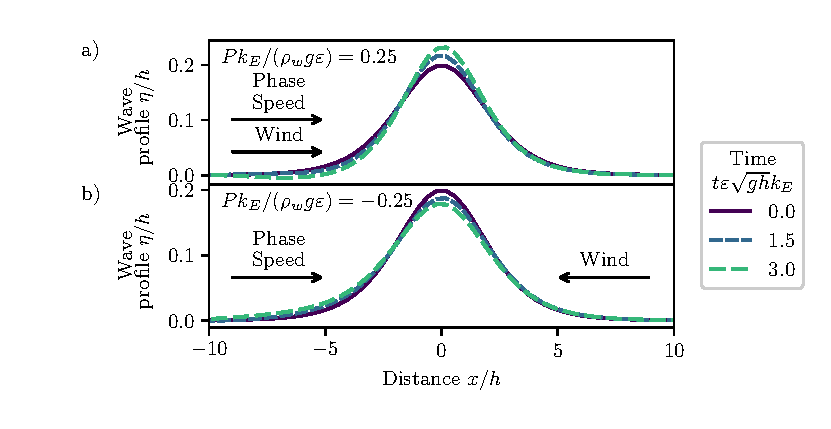
\includegraphics{Snapshots-Positive-Negative-Production.eps}
  \vspace{-0.25cm}
  \caption{
    Solitary wave evolution under
    \subref{fig:snapshots_solitary:a}
    onshore and
    \subref{fig:snapshots_solitary:b}
    offshore wind-induced surface pressure in the frame of the unforced
    solitary wave.
    Non-dimensional wave height $\eta/h$ versus
    non-dimensional distance $x/h$ for $\epsilon=0.1$,
    $\mu_E = 0.6$, $\abs{P k_E/(\rho_w g \epsilon)} = 0.25$, and
    non-dimensional slow times $t'_1 = t \epsilon \sqrt{gh} k_E = 0$,
    $1.5$ and $3$, as indicated in the legend.
    Only a subset of the full spatial domain is shown.
    The arrows denote the wave propagation (phase speed) and wind
    direction.
  }\label{fig:snapshots_solitary}
\end{figure}

The wave profile $\eta/h$ snapshots in \cref{fig:snapshots_solitary}
qualitatively show how the wave shape evolves over non-dimensional slow
time $t'_1 = t \epsilon \sqrt{g h} k_E$ when plotted against the
non-dimensional distance $x/h$ in the unforced solitary wave's frame.
First, the onshore wind generates wave growth, apparent at the wave
crest $x=0$ (\cref{fig:snapshots_solitary:a}), while the onshore wind
causes wave decay (\cref{fig:snapshots_solitary:b}).
The wind also slightly changes the phase speed, with the wave's
acceleration (deceleration) under an onshore (onshore) wind visible by
the slight advancing (receding) of the crest.
This is expected due to the phase speed's dependence on the
growing/decaying wave height \cref{eq:initial_condition}.
Additionally, despite the wave starting from a symmetric, solitary-wave
initial condition, the wind induces a horizontal asymmetry in the wave
shape, particularly on the rear face ($x<0$) of the wave.
The offshore wind (\cref{fig:snapshots_solitary:b}) raises the
rear base of the wave (near $x/h = -6$) relative to its initial profile
(purple line), but the onshore wind (\cref{fig:snapshots_solitary:a})
depresses the rear face and forms a small depression below the still
water level at $t\epsilon \sqrt{gh} k_E=3$ (green line).
Additionally, the onshore wind (\cref{fig:snapshots_solitary:a})
increases the maximum wave-slope magnitude with time while the offshore
wind (\cref{fig:snapshots_solitary:b}) decreases it, though the windward
side of the wave becomes steeper than the leeward side for both winds
(up to \SI{8}{\percent} steeper for the time period shown).

\begin{figure}
  \centering
  { % Put \phantomsubcaption in their own group to prevent it from
    % affecting the main figure's numbering
    \phantomsubcaption{}\label{fig:snapshots_solitary_tail:a}
    \phantomsubcaption{}\label{fig:snapshots_solitary_tail:b}
  }
  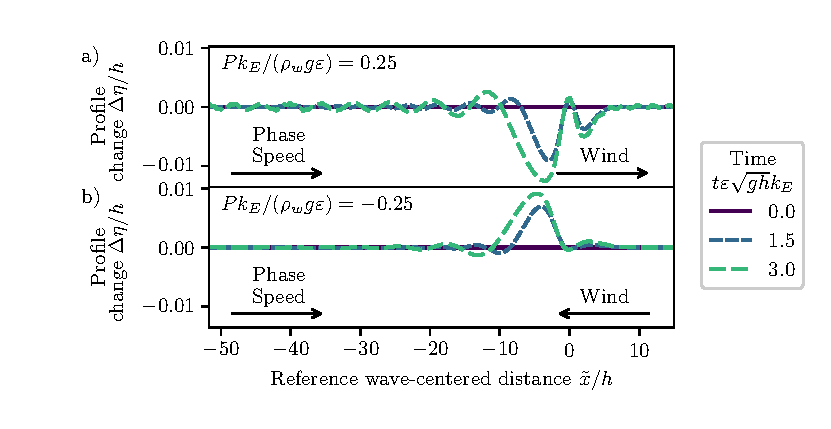
\includegraphics{Snapshots-Positive-Negative-Tail.eps}
  \vspace{-0.25cm}
  \caption{
    The non-dimensional profile change $\Delta \eta/h$ between the
    surface profile and reference solitary wave
    \cref{eq:initial_condition} under
    \subref{fig:snapshots_solitary_tail:a} onshore and
    \subref{fig:snapshots_solitary_tail:b} offshore Jeffreys forcing
    versus non-dimensional reference wave-centered distance
    $\tilde{x}/h$.
    Results are shown for $\epsilon=0.1$, $\mu_E = 0.6$, $\abs{P
    k_E/(\rho_w g \epsilon)} = 0.25$, and non-dimensional slow times
    $t'_1 = t \epsilon \sqrt{gh} k_E = 0$, $1.5$ and $3$, as indicated
    in the legend.
    Only a subset of the full spatial domain is shown.
    The arrows denote the direction of wave propagation (phase speed) or
    wind direction.
  }\label{fig:snapshots_solitary_tail}
\end{figure}

To further examine the wind-induced wave asymmetry, we fit $\eta$ to a
solitary wave profile $\eta_{\text{ref}}$ \cref{eq:initial_condition} by
minimizing the $L_1$ difference.
This gives the reference solitary wave's height $H_{\text{ref}}(t_1)$
and peak location $x_{\text{ref}}(t_1)$.
We subtract the reference solitary wave with the appropriate height from
the profile and plot the profile change $\Delta \eta(x) \coloneqq \eta -
\eta_{\text{ref}}$ as a function of the reference wave-centered distance
$\tilde{x} \coloneqq x - x_{\text{ref}}$ in
\cref{fig:snapshots_solitary_tail}.
Notice that the profile change begins near the front face of the wave
and has extrema for negative $\tilde{x}'$ but with opposite signs for
onshore and offshore winds.
Additionally, the magnitude of the extrema decay quickly with distance
in the $-\tilde{x}$ direction.
Finally, note that the onshore (offshore) wind generates a small peak
(trough) at $\tilde{x} = 0$ and two small troughs (peaks) near
$\tilde{x}/h = \pm 3$, with the $\tilde{x}<0$ extrema larger than the
$\tilde{x}>0$ one.

\begin{figure}
  \centering
  { % Put \phantomsubcaption in their own group to prevent it from
    % affecting the main figure's numbering
    \phantomsubcaption{}\label{fig:statistics_solitary:a}
    \phantomsubcaption{}\label{fig:statistics_solitary:b}
    \phantomsubcaption{}\label{fig:statistics_solitary:c}
  }
  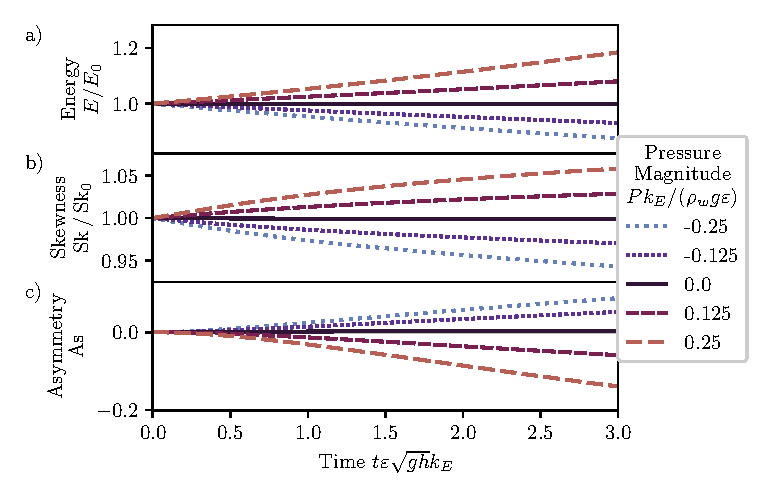
\includegraphics{Skew-Asymm-Production.eps}
  \vspace{-0.25cm}
  \caption{
    Solitary wave shape statistics under onshore and offshore
    Jeffreys forcing versus non-dimensional slow time $t'_1 = t
    \epsilon \sqrt{gh} k_E = \numrange{0}{3}$.
    The
    \subref{fig:statistics_solitary:a}
    energy (normalized by the initial energy),
    \subref{fig:statistics_solitary:b}
    skewness (normalized by the initial skewness) and
    \subref{fig:statistics_solitary:c}
    asymmetry are defined in
    \cref{eq:shape_stats_def}.
    Results are shown for $\epsilon=0.1$, $\mu_E = 0.6$ and pressure
    magnitude $P k_E/(\rho_w g \epsilon)$ up to $0.25$, as indicated in
    the legend.
    The solid black line is the unforced case, $P = 0$, and
    shows no growth or asymmetry and a constant skewness.
  }\label{fig:statistics_solitary}
\end{figure}

The effect of wind on wave shape is quantified by the time evolution of
wave shape statistics---energy, skewness and asymmetry---for onshore
and offshore wind~(\cref{fig:statistics_solitary}).
We plot all cases for initial steepness $\epsilon = 0.1$ up to slow time
$t \epsilon \sqrt{g h} k_E = 3$, corresponding to $3/\epsilon = 30$
wave-crossing times, $\sqrt{gh} k_E$.
The unforced case ($P=0$) displays constant shape statistics and zero
asymmetry, as expected.
The normalized energy $E/E_0$ shows different growth/decay rates:
the onshore wind ($P>0$) causes accelerating wave growth while the
offshore wind ($P<0$) causes slowing wave decay
(\cref{fig:statistics_solitary:a}), which was also visible in the crest
growth/decay of \cref{fig:snapshots_solitary}.
The onshore (offshore) wind causes the wave to become more (less) skewed
over time, with the normalized skewness nearly symmetric about unity
with respect to $\pm P$.
Finally, the onshore wind causes a backwards tilt and negative asymmetry
while the offshore wind increases the asymmetry and causes a forward
tilt, which was also seen in \cref{fig:snapshots_solitary}.
Notice that $\abs{\As}$ is larger for onshore winds than offshore winds.
Since the definitions of the skewness and asymmetry are insensitive to
waveform scaling $\eta \to \lambda \eta$, this effect is not simply
caused by the wave's growth/decay.
Instead, the onshore wind generates a larger oscillatory tail
(\cref{fig:snapshots_solitary_tail}), which is the asymmetric wave
component.

\vspace{-0.5cm}
\section{\label{sec:discussion} Discussion}

\subsection{\label{sec:press_mag} Wind speed estimation}
We now relate the non-dimensional pressure magnitude $P k_E/(\rho_w g) =
\order{\epsilon}$ to the wind speed.
First, we need a relationship between the surface pressure and wave
energy $E$ \cref{eq:shape_stats_def}, which we can approximate using the
standard procedure \citep[\eg][]{mei2005nonlinear} of multiplying the
(non-dimensional, denoted by primes) KdV-Burgers equation
\cref{eq:kdv_burgers} by $\eta'_0$ and integrating from $x'=-\infty$ to
$\infty$ to obtain
\begin{equation}
  \pdv{t'_1} \int_{-\infty}^{\infty} {\eta'}_0^2 \dd{x'}
  = \int_{-\infty}^{\infty} P' \pqty{\pdv{\eta'_0}{x'}}^2
  \dd{x'} \,.
\end{equation}
The left integral is the non-dimensional energy
\cref{eq:shape_stats_def}, so re-dimensionalizing and converting back to
the full time $t$ gives the energy growth rate $\gamma$,
\begin{equation}
  \frac{\gamma}{c k_E} \coloneqq
  \frac{1}{c k_E E} \pdv{E}{t}
  = \frac{P k_E}{\rho_w g} \frac{\langle (\partial_x \eta)^2 \rangle}
    {\langle (k_E \eta)^2 \rangle}
  = \frac{1}{5} \frac{P k_E}{\rho_w g}
  \,,
  \label{eq:gamma_vs_P_solitary}
\end{equation}
with $c = \sqrt{gh}$ the phase speed and the angle brackets evaluated
with the initial, solitary wave profile \cref{eq:initial_condition}.
Alternatively, we can numerically fit the energy growth rate to
\begin{equation}
  E \propto \frac{1}{\pqty{1 - \gamma t}^2}
  \qq{with}
  \gamma \coloneqq b \bqty{\frac{P k_E}{\rho_w g}} c k_E
  \,,
  \label{eq:actual_energy}
\end{equation}
resulting in $b = \num{0.10000 \pm 0.00009}$.
\Cref{eq:actual_energy} has the same functional form and similar growth
rate $\gamma = (2/15) (P k_E/\rho_w g \epsilon) ck$ to that derived for
solitary waves using a secondary multiple-scale approximation of the
KdV-Burgers equation~\citep{zdyrski2019effects}.
Note that the exponential energy growth \cref{eq:gamma_vs_P_solitary}
correctly approximates the rational energy growth
\cref{eq:actual_energy} for small times $\gamma t \ll 1$,
and both expressions are consistent with the observed accelerating
(decelerating) energy change for $P>0$ ($P<0$) in
\cref{fig:statistics_solitary}.

Next, \citeauthor{jeffreys1925formation}'s
\citeyearpar{jeffreys1925formation} theory relates the growth rate of
periodic waves to the wind speed $U_{\lambda/2}$,
measured at a height equal to half the wavelength $z=\lambda/2$, as
\begin{equation}
  \frac{\gamma}{c k} = S_{\lambda/2} \frac{\rho_a}{\rho_w}
    \pqty{\frac{U_{\lambda/2}}{c}-1}
    \abs{\frac{U_{\lambda/2}}{c}-1} \,,
  \label{eq:gamma_vs_u_jeffreys}
\end{equation}
with $S_{\lambda/2}$ a small, non-dimensional sheltering parameter
potentially dependent on $\epsilon$, $\mu_E$ and $U_{\lambda/2}/c$.
Combining this with \cref{eq:gamma_vs_P_solitary} gives
\begin{equation}
  U_{\lambda/2} = c \pqty{1 \pm \sqrt{\frac{1}{5} \abs{\frac{P k_E}{\rho_w g}}
    \frac{\rho_w}{\rho_a} \frac{1}{S_{\lambda/2}}}} \,.
  \label{eq:U_vs_P}
\end{equation}
Here, the $\pm$ corresponds to onshore ($+$) or offshore ($-$) winds.
Note that changing the wind direction (\ie{} $\pm$ sign) while holding
the surface pressure magnitude $\abs{Pk_E/(\rho_w g)}$ constant means
onshore wind speeds $\abs{U_{\lambda/2}}$ will be larger than offshore
wind speeds.

We can evaluate \cref{eq:U_vs_P} for the parameters of
\cref{sec:results}: $\epsilon=0.1$, $\mu_E = 0.6$ and $Pk/(\rho_w g
\epsilon) = 0.25$.
\Citet{donelan2006wave} parameterized $S_{\lambda/2}$ for
periodic shallow-water waves with a dependence on airflow separation:
$S_{\lambda/2} = 4.91 \epsilon \sqrt{\mu}$ for our non-separated
flow (according to their criterion), with $\mu \coloneqq (kh)^2$.
Assuming this holds approximately for solitary waves, we choose $\lambda
= 2 \pi/k_E = \SI{20}{\meter}$ to calculate the wind speed at $z
= \lambda/2 = \SI{10}{\meter}$.
This choice corresponds to a depth of $h = \SI{2.5}{\meter}$ and initial
wave height $H_0 = \SI{0.5}{\meter}$ and yields a wind speed of $U_{10}
= \SI{21}{\meter\per\second}$, a physically realistic wind speed for
strongly forced shallow-water waves.
Weaker wind speeds will induce smaller surface pressures and thus take
longer to change the wave shape.

\subsection{\label{sec:physical_reason} Physical mechanism of asymmetry
generation}
Our initial, symmetric solitary waves \cref{eq:initial_condition} are
permanent-form solutions of the unforced KdV equation, so the pressure
forcing term in the KdV-Burgers equation is responsible for the wave
growth/decay and resultant shape changes and asymmetry, though not
directly.
Indeed, when the surface profile $\eta$ is symmetric, the pressure
forcing term $P \partial_x^2 \eta$ preserves this symmetry.
Instead, the pressure forcing causes a (symmetric) bound wave after a
short time $\Delta t'_1 \ll 1$, which can be seen by considering the
non-dimensional KdV-Burgers equation \cref{eq:kdv_burgers} in the
unforced solitary wave's frame (\cref{fig:snapshots_solitary}) at the
initial time,
\begin{align}
  &\eval{\pdv{\eta'_0}{t_1}}_{t'_1=0} = -P' \pdv[2]{x} \bqty{
  \sech^2\pqty{\frac{x'}{2}}}
  \\
  &\quad \implies \eta'_0(x', \Delta t'_1) =
  (2-P'\Delta t'_1) \sech^2\pqty{\frac{x'}{2}}
  +
  P' \Delta t'_1 \frac{3}{2}\sech^4\pqty{\frac{x'}{2}}
  \,.
  \label{eq:pressure_change}
\end{align}
The $P'\Delta t'_1$ terms generate a small peak (trough) at $x'=0$ and
small troughs (peaks) symmetrically in front and behind the wave peak
for onshore (offshore) wind; these are apparent in
\cref{fig:snapshots_solitary_tail} near $\tilde{x}/h \approx \pm 3$.
The small numerical value $\abs{P'} = 0.25 \ll 1$ used in
\cref{sec:results} allows us to consider the wave's evolution as two
steps with time scale separation.
First, the pressure modifies the wave \cref{eq:pressure_change} on the
slow time scale, and then the wave evolves on fast time scale from this
new profile according to unforced KdV evolution.
This evolution is described by the inverse scattering transform, which
shows that any localized, initial profile differing from
\cref{eq:initial_condition} will split into discrete solitary waves and
an oscillatory tail that decays behind ($x<0$) the wave
\citep[\eg][]{mei2005nonlinear}.
Prior studies on shallow-water, KdV solitary waves have also noted this
ubiquitous oscillatory tail, such as \figsname{} 8(b) and (c) of
\citet{hammack1974korteweg}.
Hence, the symmetric disturbance induced by the pressure forcing
\cref{eq:pressure_change} has two effects on the wave.
First, it slowly changes the height and width of the initial solitary
wave, which is reflected in the growth (decay) and narrowing (widening)
under onshore (offshore) winds in \cref{fig:snapshots_solitary}.
Second, it quickly generates an asymmetric, oscillatory tail behind the
wave (\cref{fig:snapshots_solitary_tail}), producing a greater shape
change on the wave's rear face (\cref{fig:snapshots_solitary}).
Finally, the different wind directions (\ie{} pressure forcing signs)
change the sign of the oscillatory tail and, hence, the sign of the
asymmetry in \cref{fig:statistics_solitary}.

\subsection{Comparison to intermediate and deep water}
\Citet{zdyrski2020wind} investigated the effect of
wind on Stokes-like waves in intermediate to deep water.
This study, with wind coupled to waves in shallow water, finds
qualitative agreement with those intermediate- and deep-water results.
The shallow-water asymmetry magnitude increases as the pressure
magnitude $P$ increases~(\cref{fig:statistics_solitary}), and \figname{}
4(a) of \citet{zdyrski2020wind} displayed a similar trend for the
corresponding Jeffreys pressure profile, with positive (negative)
pressure increasing (decreasing) the asymmetry.
Although \citet{zdyrski2020wind} compared their theoretical
predictions to limited experimental results with $kh > 1$, there are no
appropriate experiments on wind-induced changes to wave shape in shallow
water for comparison with our results.
In addition to the Jeffreys pressure profile employed here,
\citet{zdyrski2020wind} also utilized a Generalized Miles (GM) profile,
only applicable to periodic waves, wherein the pressure was proportional
to $\eta$ shifted by a distance parameter $\psi_P/k$.
Though this analysis focuses on solitary waves, we also investigated the
effect of wind on periodic waves using the cnoidal-wave KdV solutions as
initial conditions.
The Jeffreys forcing produced shape statistics qualitatively
similar to those derived for solitary waves and were omitted for
brevity, while the GM forcing gave rise to a nonlocal KdV equation and
produced unphysical effects such as the growth of higher harmonics under
damping, offshore winds, and was therefore omitted as well.

\vspace{-0.25cm}
\section{Conclusion}
Prior results~\citep{zdyrski2020wind} in intermediate and deep water
demonstrated that wind, acting though a wave-dependent surface
pressure, can generate shape changes that become more pronounced in
shallow water.
Here, we utilized a multiple-scale analysis to couple weak wind with
small, shallow-water waves, \ie{} $a_0/h \sim (k_E h)^2 \sim P k/(\rho_w
g) \ll 1$.
This gave a KdV-Burgers equation governing the wave profile $\eta$
which was solved numerically with a symmetric, solitary wave initial
condition.
The deviations between the numerical results and a reference solitary
wave had the form of an oscillatory tail, with differing sign for
onshore and offshore wind.
The tail's presence and shape are the result of a symmetric,
pressure-induced shape change evolving under the inverse scattering
transform.
We also estimated the energy, skewness and
asymmetry as functions of time and pressure magnitude.
For onshore wind (positive $P$), wave energy and skewness increased with
time while asymmetry decreased, while offshore wind produced the
opposite effects.
Furthermore, these effects were enhanced for strong pressures, and they
reduced to the unforced case for $P=0$.
The shape statistics found here show qualitative agreement with the
results in intermediate and deep water.
Finally, the wind speeds corresponding to these pressure differences
were calculated and found to be physically realistic.

\begin{acknowledgements}
We are grateful to D.~G.~Grimes and M.~S.~Spydell for discussions on
this work.
We thank the National Science Foundation (OCE-1558695) and the Mark Walk
Wolfinger Surfzone Processes Research Fund for their support of this
work.
Declaration of Interests. The authors report no conflict of interest.
\end{acknowledgements}

\vspace{-0.5cm}
% Bibliography
\bibliographystyle{jfm}
\bibliography{references}

\end{document}
